\documentclass{article}
\usepackage{blindtext}
\usepackage[utf8]{inputenc}
\usepackage{graphicx}
\usepackage{hyperref}
\newcommand{\includegraph}[1]{\includegraphics[width=\textwidth,height=\textheight,keepaspectratio]{#1}}

\title{DeepREG}
\author{Boxiang Liu}
\date{\today}
\begin{document}
\maketitle
\tableofcontents


\section{Basset} 
The Basset architecture represent the state-of-the-art for open chromatin predictions. The architecture is as follows:

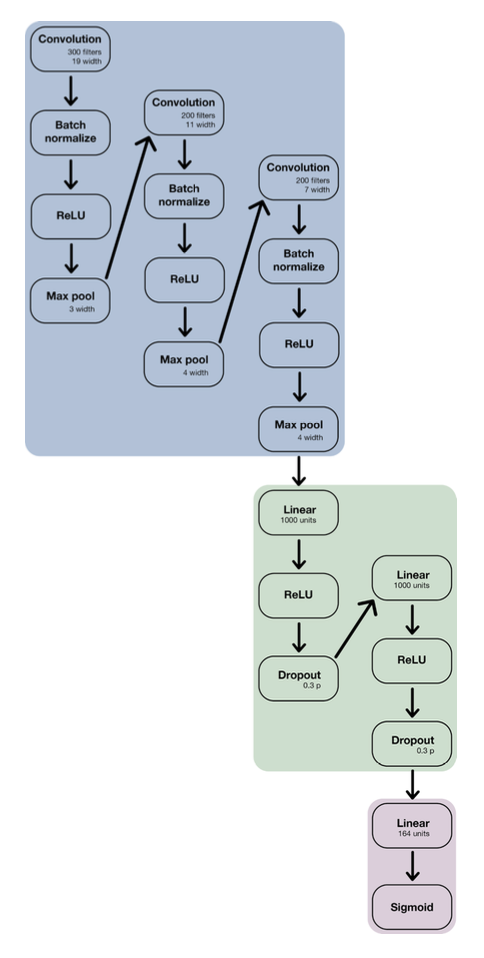
\includegraphics[width=\textwidth,height=\textheight,keepaspectratio]{modeling/basset/architecture.png}

I used it for the CNN part of the network. The detailed network graph is below: 

\includegraphics[width=\textwidth,height=\textheight,keepaspectratio]{../figures/basset/model.eps}

However, the network did not train properly, likely due to too many layers.


\section{Reducing CNN layers}
Given that 3 layers won't train, I removed one layer (in directory keras1). 

\includegraphics[width=\textwidth,height=\textheight,keepaspectratio]{../figures/keras1/model.eps}

The result is quite promising. 

\includegraphics[width=\textwidth,height=\textheight,keepaspectratio]{../figures/keras1/pred_vs_obs.png}

The first layer used filter width of 100, which is quite large.


\section{Small filter}
\label{sec:small_filter}
Since most motifs are less than 20 bps, I used a filter witdh of 19 bps. 

\includegraphics[width=\textwidth,height=\textheight,keepaspectratio]{../figures/small_filter/model.eps}

The result is as good as using 100 width filters.

\includegraphics[width=\textwidth,height=\textheight,keepaspectratio]{../figures/small_filter/pred_vs_obs.png}


\section{Single layer}
When using more than one layer, either for the seq or the regulator network, the interpretability is lost. I therefore tried using one conv layer (as motif scanner) for the seq network, and no dense layer for the reg network.

\includegraphics[width=\textwidth,height=\textheight,keepaspectratio]{../figures/single_layer/model.eps}

The model worked really well. The training loss dropped to almost zero after 30 epochs, and does not show any sign of plateau (compared to \hyperref[sec:small_filter]){small filter}). However the test loss does not decrease as much indicating overfitting. 


\includegraphics[width=\textwidth,height=\textheight,keepaspectratio]{../figures/single_layer/pred_vs_obs.png}
\includegraphics[width=\textwidth,height=\textheight,keepaspectratio]{../figures/single_layer/loss_vs_epoch.png}

Therefore I created a new model with l1 (=1e-7) and l2 (=1e-7) on all weights regularization. Although this model prevented overfitting on the training set, the test set performance actually worsened. 

\includegraph{../figures/single_layer/20170605_092542_l1_1e-07_l2_1e-07/loss_vs_epoch.png}



\subsection{Motif discovery}
Is the network find known motifs? I took top 100 sequences with largest activation for each filter and use TomTom to match them to known motifs.

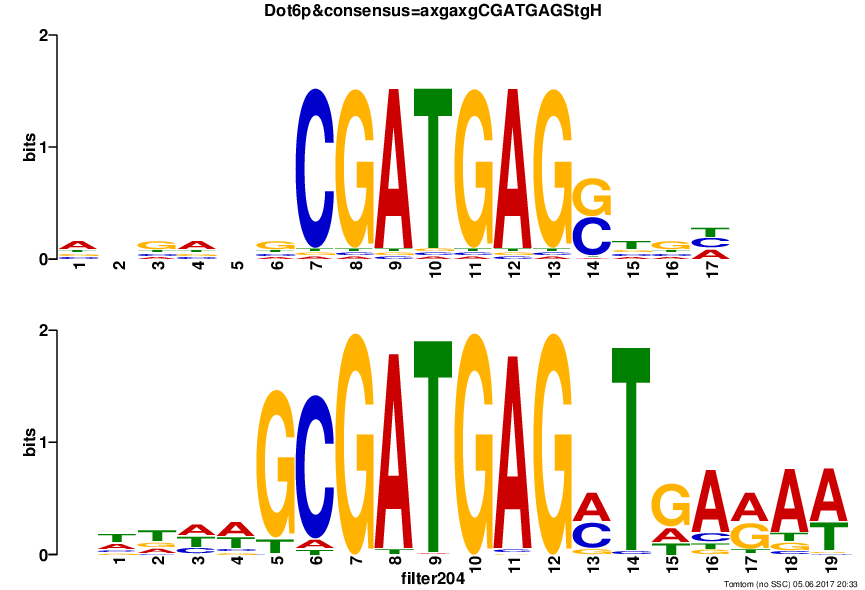
\includegraphics[width=\textwidth]{../figures/single_layer/interpret/tomtom/dot6p_2.png}
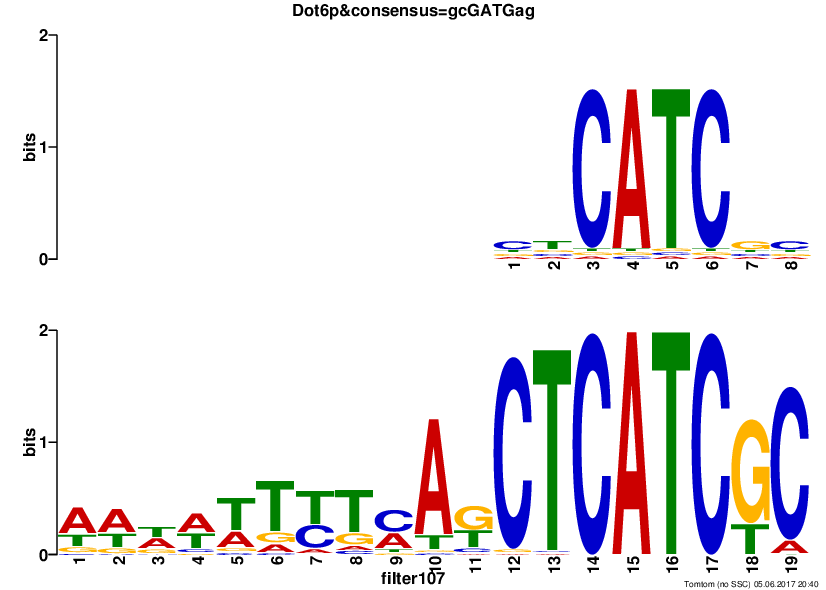
\includegraphics[width=\textwidth]{../figures/single_layer/interpret/tomtom/dot6p_3.png}
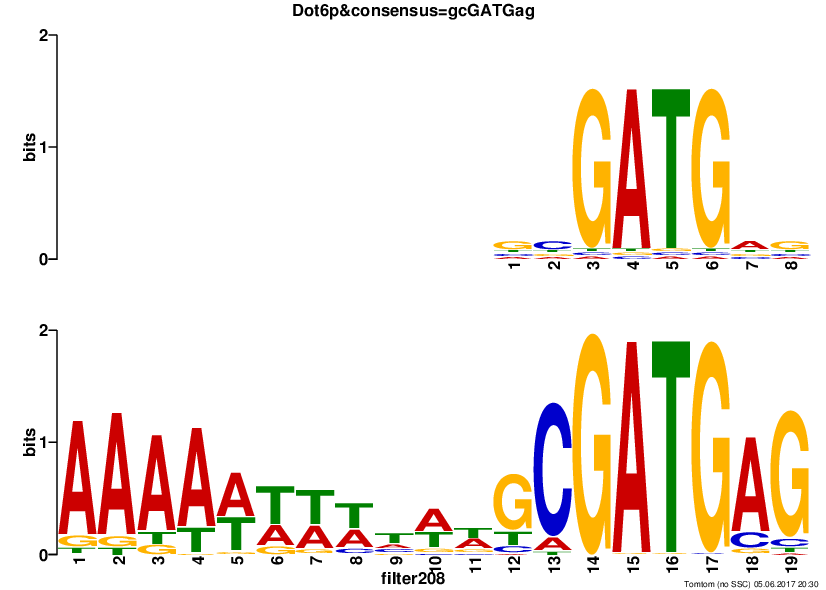
\includegraphics[width=\textwidth]{../figures/single_layer/interpret/tomtom/dot6p.png}
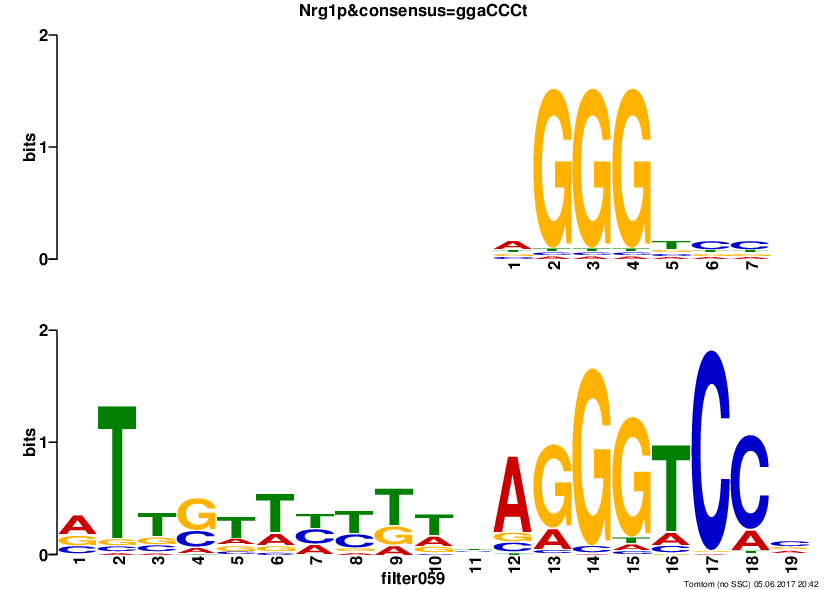
\includegraphics[width=\textwidth]{../figures/single_layer/interpret/tomtom/nrg1p.png}
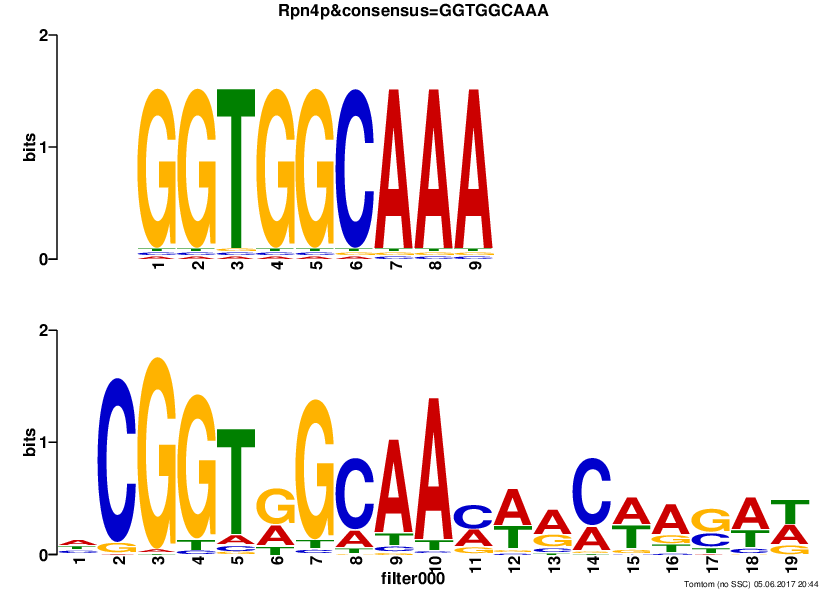
\includegraphics[width=\textwidth]{../figures/single_layer/interpret/tomtom/rpn4p.png}
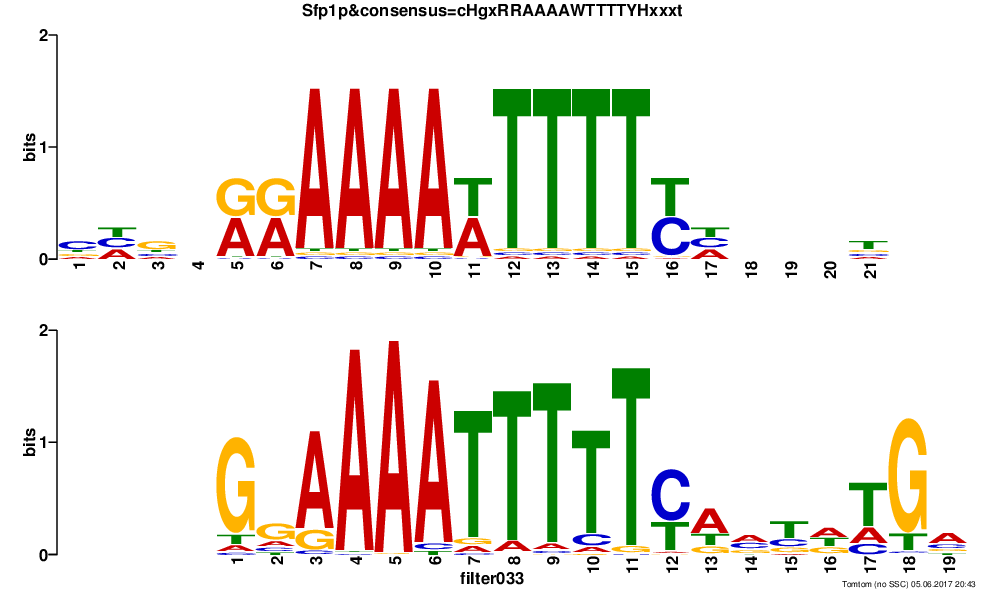
\includegraphics[width=\textwidth]{../figures/single_layer/interpret/tomtom/sfp1p_2.png}
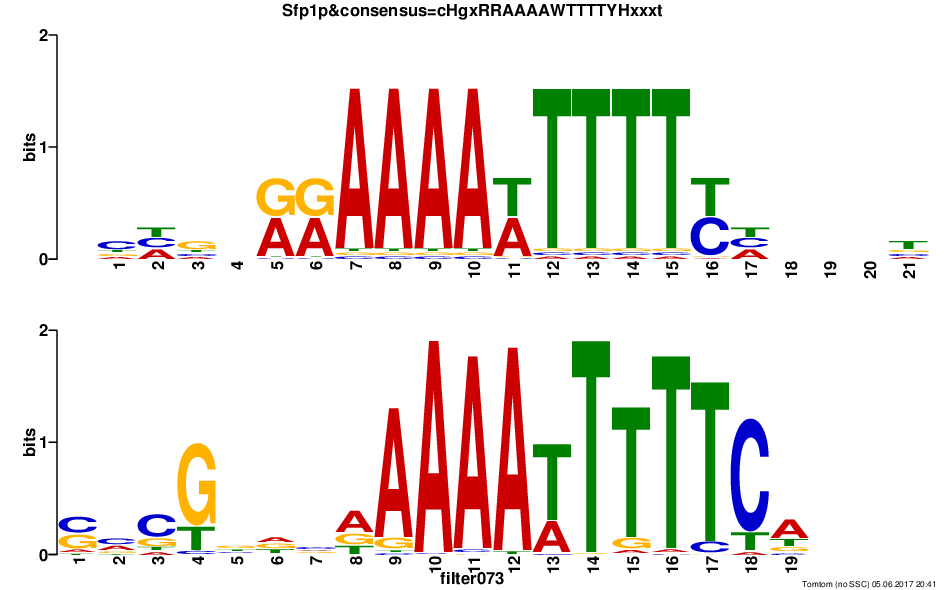
\includegraphics[width=\textwidth]{../figures/single_layer/interpret/tomtom/sfp1p.png}
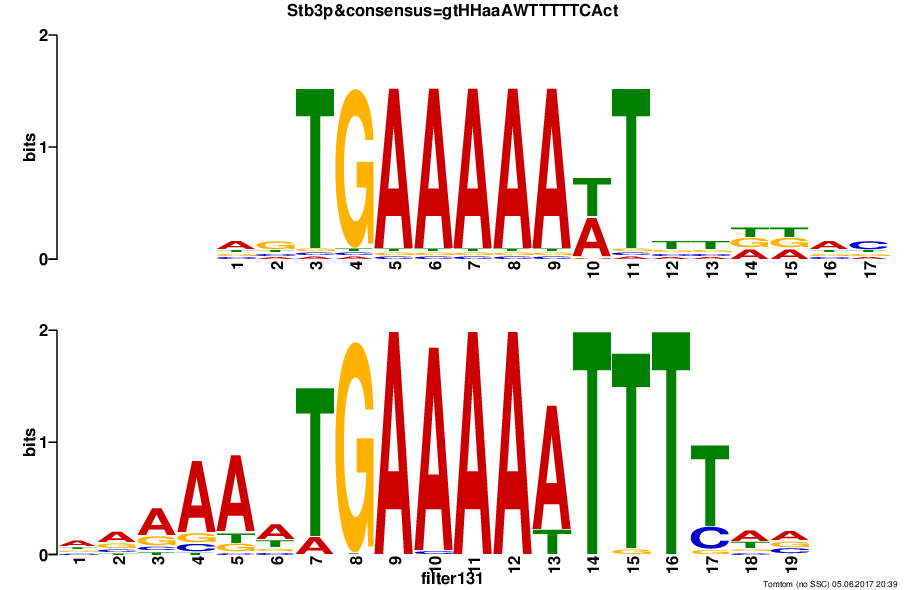
\includegraphics[width=\textwidth]{../figures/single_layer/interpret/tomtom/stb3p.png}





\end{document}
